\documentclass[10pt, a4paper]{article}
\usepackage[utf8]{inputenc}

\usepackage{amsmath,wasysym}
\usepackage{amsrefs}
\usepackage{tikz, wasysym}
\usepackage[]{csquotes}
\usepackage[utf8]{inputenc}
\usepackage[german]{babel}
\usepackage[export]{adjustbox}
\usepackage{pdfpages}

\author{Sven Fiergolla, 1252732}
\title{Portfolio zur Vorlesung Programmierung II}


\begin{document}
 

\clearpage\maketitle
\thispagestyle{empty}
\pagebreak


\section*{Reflexion}

\paragraph*{}
Zu Beginn der Vorlesungsreihe beschäftigten wir uns mit einfachen Datenstrukturen und deren Aufbau, beispielsweise verkettete Listen, binäre Bäume und Schlangen als Wiederholung. Da diese Strukturen als Grundlage für viele der weiterführenden Themen sind, ist die Behandlung dieser notwendig und hilfreich.\par

\paragraph*{}
Ebenso wurde die Funktionsweise von \textit{Interfaces, Streams} und \textit{Exeptionhandling} rekapituliert und den Studenten wurde das \textit{log4j}-Framework zum standardisierten Logging der eigenen Anwendungen erläutert und dessen Verwendung nahegelegt. Mit \textit{Streams} wurde uns die Möglichkeit zur funktionalen Programmierung in Java gegeben, ein Konzept, was im weiteren Verlauf der Vorlesung, durch die Verwendung von Skala, als funktionale Sprache, gefestigt wurde. Anständiges \textit{Exceptionhandling} und \textit{Logging} wurde zwar gelehrt, die wirkliche Bedeutung dieser Konzepte versteht man jedoch erst, wenn man eigene, größere Projekte verfasst, welche ohne jene Konzepte praktisch nicht umzusetzten sind.\par


\paragraph*{}
Anschließend beschäftigten wir uns mit graphischen Benutzeroberflächen unter Gebrauch des GUI-Toolkits \textit{SWING} und erstellten eigene Benutzeroberflächen oder Spiele (Mienenfeger aus der Vorlesung). Auch dies Thema ist von großer Bedeutung, da die meisten Endbenutzeranwendungen nicht auf eine graphische Oberflche verzichten können, um auch von unerfahrenen Anwendern genutzt werden zu können.
\par

\paragraph*{}
In den folgenden Wochen beschäftigten wir uns mit \textit{Nebenläufigkeit} in Form von mehreren Threads in einer Anwendung. Dazu animierten und simmulierten wir mehrere Kugeln auf einem Feld, welche miteinander kollidierten. Das Debuggen parallelilsierter Anwendungen stellte sich häufiger als Herrausforderung heraus, da \textit{Deadlocks}und \textit{race conditions} schwierig zu finden sind. Dennoch ist die nebenläufige Prgrammierung vorallem bei rechenintensiven und zeitkritischen Problemen vonnöten.\par

\paragraph*{}
Unter Verwendung von \textit{UDP/TCP} als Netzwerkprotokolle, lernten wir das Programmieren verteilter Anwendungen bzw. Netzwerkrogrammierung. Im Zuge dessen benutzren wir ebenfalls die Konzepte \textit{Serialisierung} und \textit{Reflection} um Java-Objekte übertragen zu können und mit diesen zu arbeiten.\\
Als Anwendung in diesem Bereich programmierten wir das Spiel \enquote{Pong} als Client-Server-Anwendung.\par

\paragraph*{}
Abschließend machten wir uns mit dem Konzept der funktionalen Programmierung vertraut und lernten dazu die Sprache Scala. Dazu arbeiteten wir mit einfachen Datenstrukturen wie Listen und Bäume und nutzen \textit{Pattern Matching} oder \textit{Currying}. Funktionale Programmierung als neues Programmierparadigma wirft eine neue Blickrichtung auf das Lösen von Problemen, da die Programme eine reine Folge von Funktionen sind. Vorallem für aktuelle Bereiche der Programmierung wie zb. neuronale Netze sind häufig funktional gelöst, was dieses Thema sehr interessant macht.\par


\section*{Einführung}
\paragraph*{}
Mein Hauptbeweggrund für die Auswahl der Aufgaben war logischerweise das Erreichen des Maximums der aufsummierten Punkte. Gleichzeitung habe ich in diesen Aufgaben das solideste Wissen, welches sich durch die erreichten Punkte widerspiegelt. Die Aufgaben die ich nicht mit einbezogen habe (die Aufgabe zur Nebenläufigkeit und die Skala-Aufgaben der großen Onlineübung) waren auch die Aufgabenbereiche in welchen ich mich am unsichersten fühlte. \par

\paragraph*{}
Onlineübung 1 und 2 als Wiederholung beeziehe ich komplett mit ein, diese Themen habe ich gut verstanden und konnte das gelernte umsetzten.\\
Von Onlineübung 3 beziehe ich nur die 1. Aufgabe (Netzwerkprogrammierung) da ich mehrere Probleme mit Aufgabe 2 (nebenläufigkeit) hatte und die Aufgabe dementsprechend ausgefallen ist.\\
Onlineübung 4 beziehe ich ebenfalls ganz mit ein, die Einführung in funktionales Programmieren war recht verständlich.\\
Von der großen Onlineübung beziehe ich nur den Java-Teil mit ein (Aufgabe 1-3) da ich mich darauf am konsequenesten vorbereitet habe und mein Verständnis in diesem Aufgabenbereich am solidesten ist.\par


\pagebreak
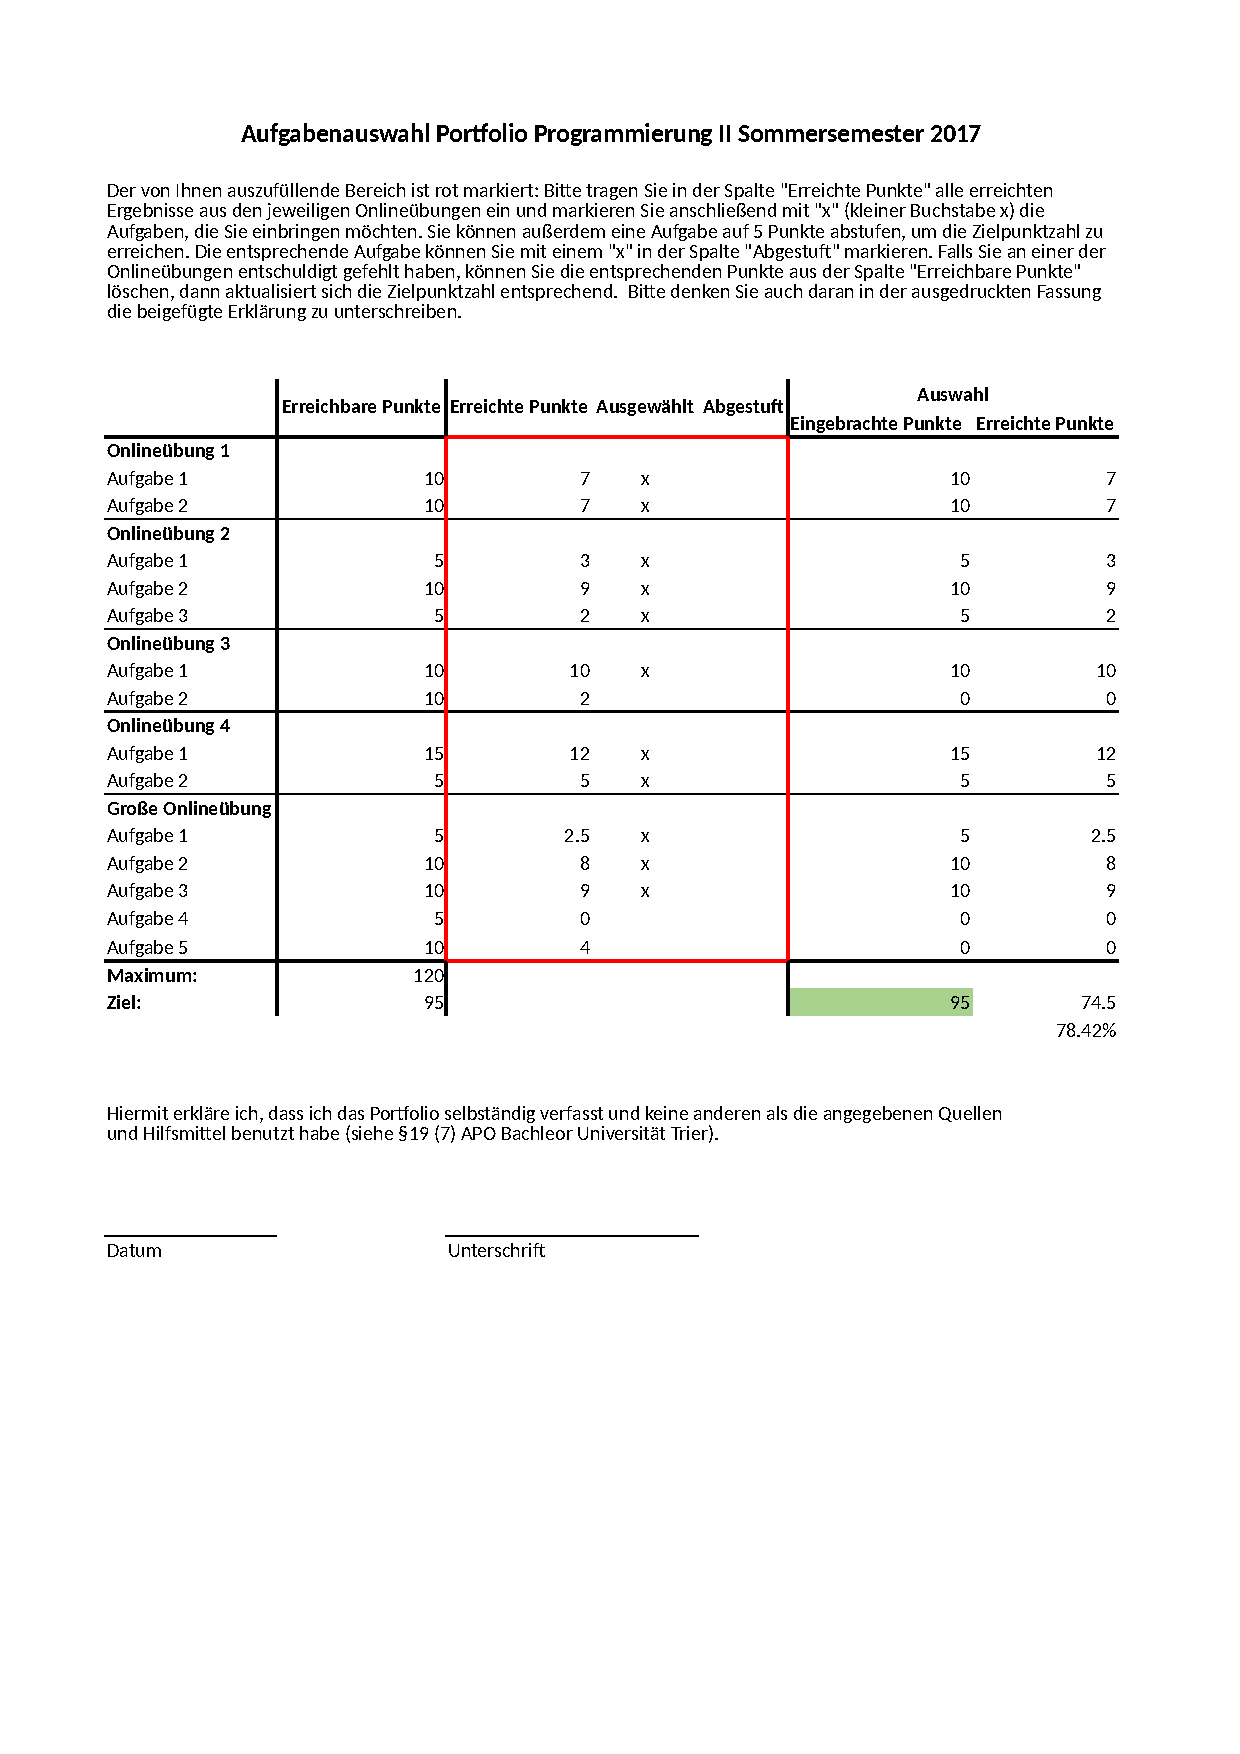
\includepdf[scale=1]{Aufgabenauswahl_Portfolio_FINAL.pdf}



\end{document}